\documentclass[14pt]{article}
\usepackage{amsmath}
\usepackage{listings} % For writing code see http://ctan.org/pkg/listings
\usepackage{graphicx}
\usepackage{float}
\usepackage[margin=1.0in]{geometry}
\usepackage{mdframed}
\usepackage{hyperref}

\title{CS665 HW3: Solutions}
\author{Nicolas Garavito-Camargo}
\begin{document}
\maketitle

\section{Part I}

\begin{mdframed}
\textbf{1.} Let $x_1, $ be $n$ points in d-dimensional  space  and  let
$X$ be the $n\times d$ matrix whose rows are the
$n$ points.  Suppose we know only the matrix $D$
of pairwise distances between points and not the coordinates of the points
themselves.  The set of points $x x_n$  giving  rise  to  the  distance  matrix
$D$ is  not  unique  since  any  translation,
rotation,  or  reflection  of  the  coordinate  system  leaves  the
distances  invariant.   Fix  the origin  of  the  coordinate  system  so  that  the  centroid  of  the
set  of  points  is  at  the  origin. That is, $\sum_i=1^n x_i = 0$

\begin{enumerate}
\item Show that the elements of $XX^T$ are given by:

\begin{equation}
x_i x_j^T = - \dfrac{1}{2} \left[ d_{ij}^2 - \dfrac{1}{n} \sum_{j=1}^n
d_{ij}^2 - \dfrac{1}{n}\sum_{i=1}^n d_{ij}^2 + \dfrac{1}{n^2}
\sum_{i=1}^2 \sum_{j=1}^n d_{ij}^2 \right]
\end{equation}

\item Describe an algorithm for determining the matrix $X$ whose rows
are the $x_i$.

\end{enumerate}

\end{mdframed}

\textbf{Solution:}\\

\textbf{1a.} The distance matrix $D$ with components $d_{ij}^2$ is defined as:

\begin{equation}
d_{ij}^{2} = (\sum_{i} x_{i})^2 + (\sum_{j} x_{j})^2 - 2 \sum_{i,j} x_i
x_j
\end{equation}

Which at the origin of the coordinate system it would be:

\begin{equation}\label{eq:dij}
d_{ij}^{2} =  - 2 \sum_{i,j} x_i x_j
\end{equation}

On the other hand the matrix $xx^T$ is:

\begin{equation}
x x^T_{ij} = (x_i - \dfrac{1}{n}\sum_i x_i )(x_j - \dfrac{1}{n}\sum_j
x_j )
\end{equation}

Doing the products the components of the matrix are:

\begin{equation}\label{eq:xxt}
xx^T_{ij} =  \sum_{ij}^n x_i x_j - \dfrac{1}{n} \sum_i x_i x_j -
\dfrac{1}{n}\sum_j x_i x_j + \dfrac{1}{n^2} \sum_{ij} x_i x_j 
\end{equation}

Using the results of Eq. \ref{eq:dij} into Eq. \ref{eq:xxt} $xx^T$ is:

\begin{equation}
xx^T_{ij} =  -\dfrac{1}{2} \left[  d_{ij}^2 - \dfrac{1}{n}
\sum_i d_{ij}^2 -
\dfrac{1}{n}\sum_j d_{ij}^2 + \dfrac{1}{n^2} \sum_{ij} d_{ij}^2 \right]
\end{equation}

Which is the desired result.\\

\textbf{1b.}\\ 

In order to determine $X$ from $D$ we need to center the matrix $D$
with a centering matrix $C$ this is:

\begin{equation}
B = -\dfrac{1}{2} C^T D C
\end{equation}

Where the factor $-1/2$ comes from equation \ref{eq:dij}, Now
computing the SVD of $XX^T = U\Sigma V^T V \Sigma U^T = U \Sigma^2
U^T$. Therefore, the eigenvalues and eigenvectors of the matrix $B$
can be computed to derive $X$ as:

\begin{equation}
X = E (\lambda I)^{1/2}
\end{equation}

Where $\lambda$ are the eigenvalues of $B$ and $E$ is the matrix of
eigenvectors.

\begin{mdframed}

\textbf{2.} Implement the algorithm you described above, and use the first two
columns of the result matrix to display the best two-dimensional
projection of the 312 points of this dataset. This dataset contains
the pairwise distances between each of 312 cities in North America.
You should be able to easily see the general shape of the continental
US, and more.

\end{mdframed}

\textbf{Solution:}\\

Implementing the classical MDS algorithm for the given data set allow
to recover 2D map of US. This is shown in figure \ref{fig:usmap}.
\textbf{All the code used to solve this homework including the plots
can be found} \href{https://nbviewer.jupyter.org/github/jngaravitoc/Lecture_notes_UofA/blob/master/DataScience/HWs/HW3.ipynb}{here}.

\begin{figure}[H]
\centering
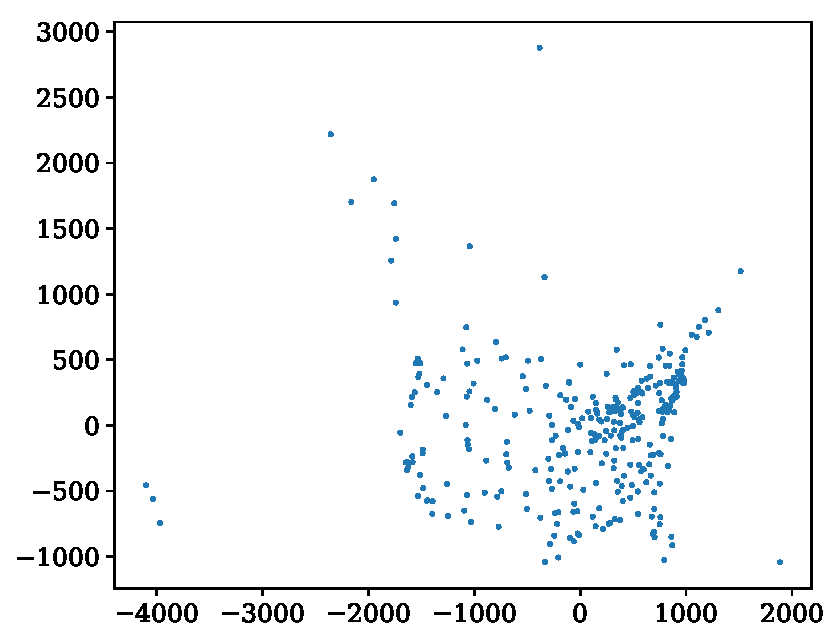
\includegraphics[scale=0.5]{usa_map.pdf}
\caption{ US map recovery from the implementation of the classical MDS
algorithm \label{fig:usmap}}
\end{figure}

\section{Part II}

\begin{mdframed}
\textbf{1.} Plot the points in two dimensions using the MDS algorithm you
implemented. Use color to encode the value associated with each data
point. You should see an outer ring of points and a smaller, inner
cluster of points. The outer points all have the value 10 associated
with them, and the inner points have the value 5 associated with them.
\end{mdframed}


\textbf{Solution:}\\

 Figure \ref{fig:rings} shows the rings in different
colors representing the different values associated with the points.

\begin{figure}[H]
\centering
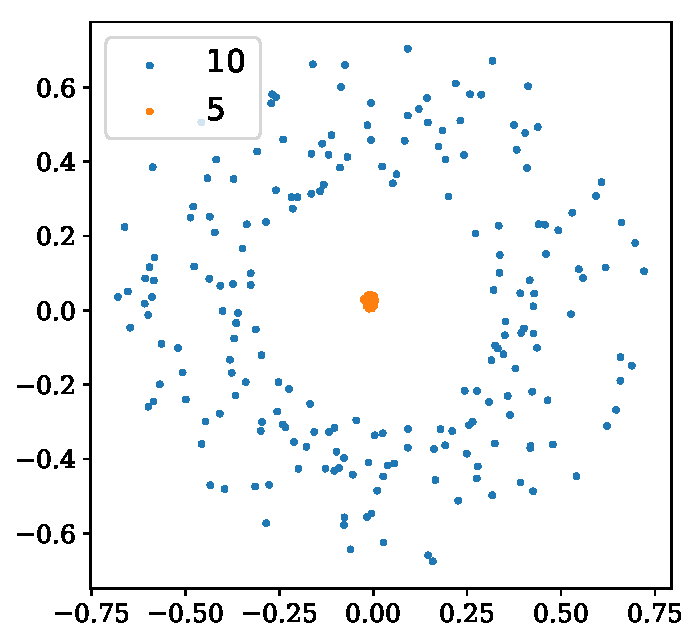
\includegraphics[scale=0.5]{rings.pdf}
\caption{ Two dimension scatter plot using the classical MDS
alogorithm, using a color code in which blue represents data with
value 10 and orange data with value 5. \label{fig:rings}}
\end{figure}

\begin{mdframed}
\textbf{2.} A natural question to ask when using MDS is: how faithful
is this plot? In other words: are two dimensions enough? Did the plot
throw away too much information? How can you use the SVD of M to
answer this question?
\end{mdframed}


\textbf{Solution:}\\

In this particular case 2D are enough number of dimensions. 
The reason is that when you
look at the $SVD$ of $M$ you find that the main principal axis
(eigenvectors) whose length are given by the values of the eigenvalues
are two. This can be seen in the figure bellow where the dots
represent the values of the eigenvalues of $M$, taking into account
the first 2 eigenvalues (i.e just two dimensions) the $99.9\%$ (this is
just $(\lambda_1 + \lambda_2) / \sum_i \lambda_i$) of the
information is recovered, therefore, this is a good recovery of the
data. In conclusion looking at the $SVD$ is very
useful to figure out how many dimensions should be used in order to
capture most of the information from a data set.


\begin{figure}[H]
\centering
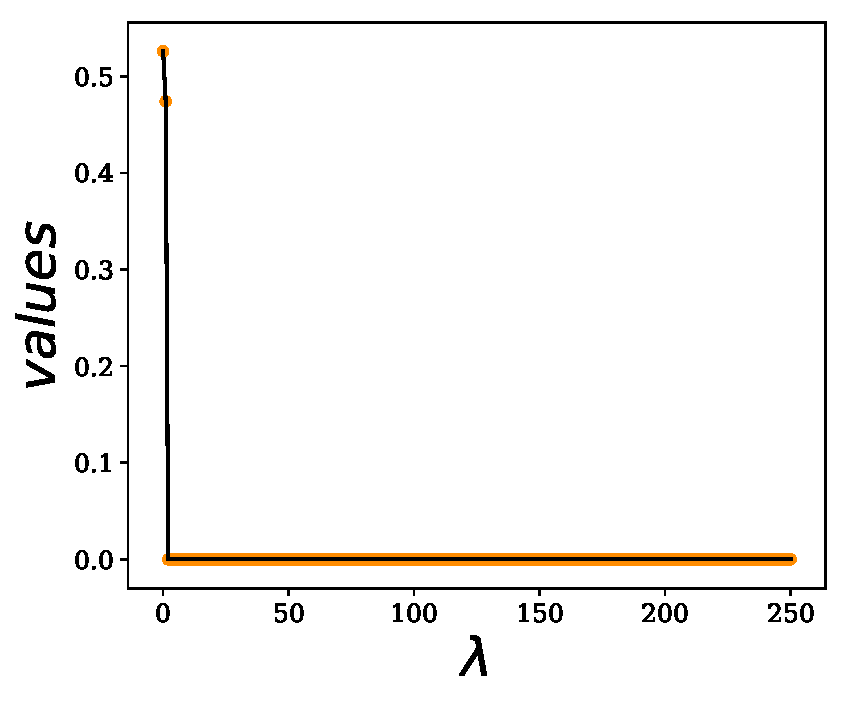
\includegraphics[scale=0.5]{M_eigval.pdf}
\caption{ Normalized eigenvalues of $M$, there are three eigenvalues whose values
are large enough, this is whose sum is closer to $1$.}
\end{figure}

\newpage

\begin{mdframed}
\textbf{3.} Implement Kernel Least Squares (KLS), and use it to solve for the
values in a 50-point testing set below (use a small $\lambda$, such as
$10\times^{−4}$). The testing points come from the same source as the training set,
so they will either be from the outer ring or the inner circle.

In Kernel Least Squares, points in the testing set are represented
implicitly by the inner products with all the points in the training
set. If we compute those values for each point in the testing set and
each point in the training set, we get a matrix. That matrix is here.

Use this matrix and KLS to compute predictions, and compare your
predictions to the ground truth. Do you get good predictions?

Why not? Can you figure out what is happening by investigating the
kernel matrix and its SVD?
\end{mdframed}


Figure \ref{fig:k1} shows the results of the predicted values
using the KLS algorithm. The predicted values are distributed over a
range of $[-2, 2]$ this is not a very good prediction. By looking at
the singular values of the kernel matrix figure \ref{fig:svds}


\begin{figure}[H]
\centering
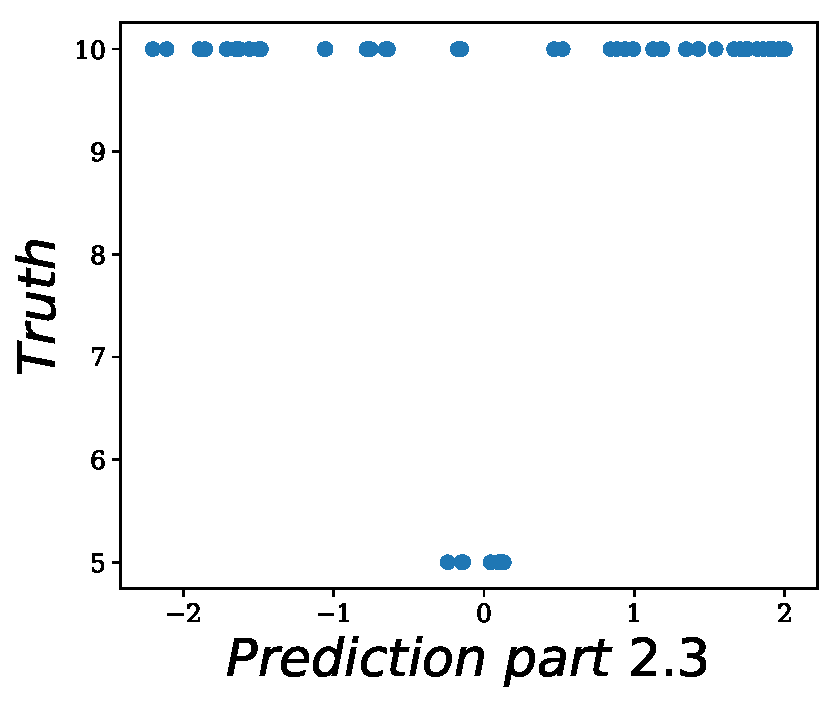
\includegraphics[scale=0.5]{kernel1.pdf}
\caption{ Truth vs predicted values using a linear
kernel.\label{fig:k1}}
\end{figure}



\begin{mdframed}
\textbf{4.} We will now use different kernel matrices to solve the same problem.
First, solve the same problem as before, but add 1
to every entry in $M$ (in other words, use a matrix $M'$, where
$m'_{ij}=m_{ij}+1$). What results do you get? Where have they improved, but
where have they not improved? Hint: remember that $m_{ij}=<v_i,v_j>$, for
some hypothetical vector representation. Remember that transforming
kernels is the same thing as transforming the representations. Relate
this transformation to what you would get if you were solving a
“normal” least squares problem. What is the difference between these
representations?

\end{mdframed}


\begin{figure}[H]
\centering
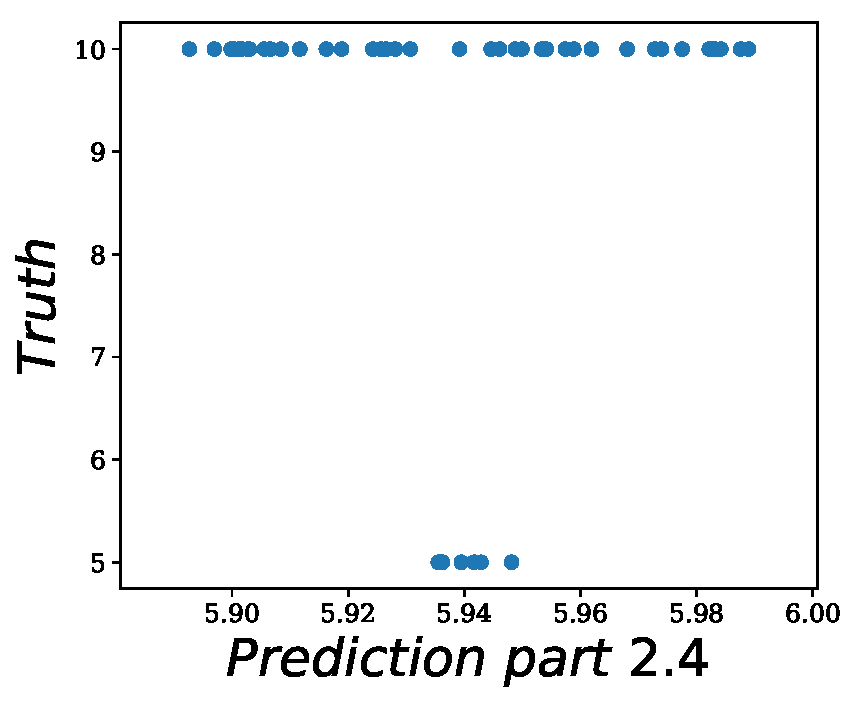
\includegraphics[scale=0.5]{kernel2.pdf}
\caption{ Truth vs predicted values using \label{fig:k2}}
\end{figure}

\begin{mdframed}
\textbf{5.} Finally, create a $M''$ matrix where $m''_{ij}=(m_{ij}+1)^2$, and use it to solve
the Kernel Least Squares problem. What results do you get now? Why are
these better?
\end{mdframed}


\begin{figure}[H]
\centering
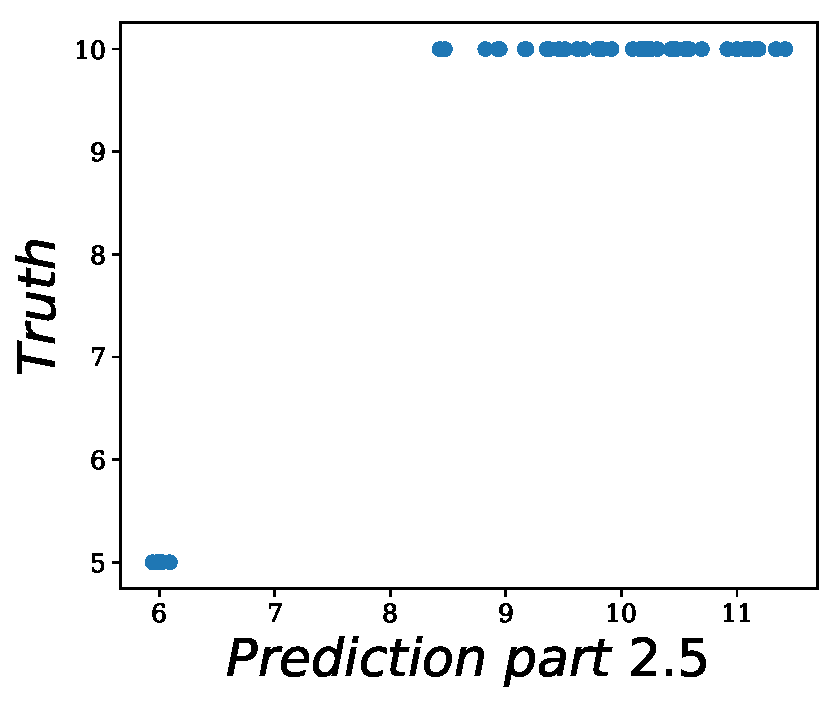
\includegraphics[scale=0.5]{kernel3.pdf}
\caption{ Normalized eigenvalues of $M$, there are three eigenvalues whose values
are large enough, this is whose sum is closer to $1$.}
\end{figure}


\begin{figure}[H]
\centering
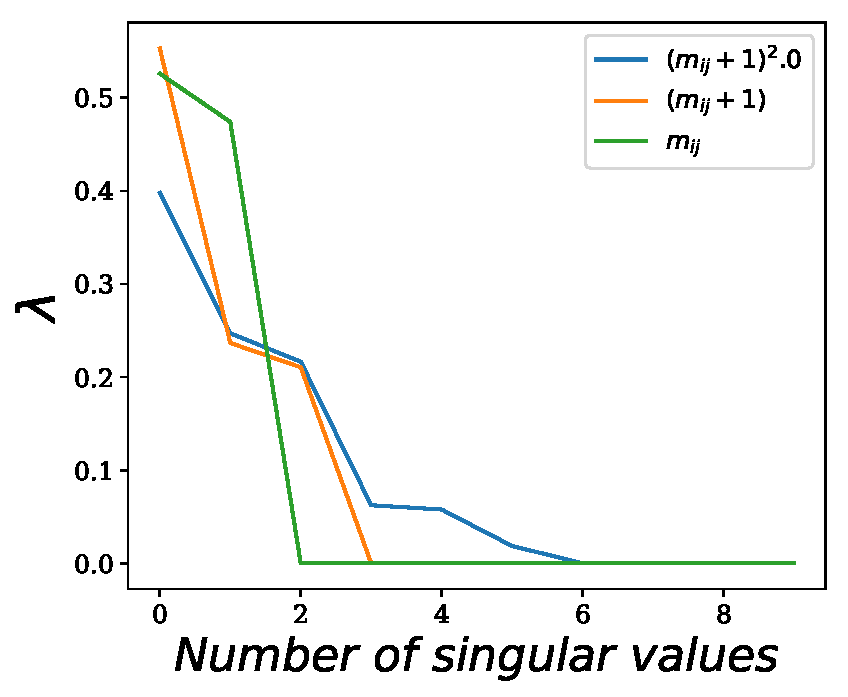
\includegraphics[scale=0.5]{SVDs_kernels.pdf}
\caption{ Singular values of the 3 different kernel
matrices.\label{fig:svds}}
\end{figure}

\end{document}
